\section{Private Empirical Risk Minimization}
 
如图\ref{fig:privacy_data_accuracy}, 在考虑个人隐私的情况下,数据集大小,隐私水平和精确度是机器学习模型训练需考虑的三个变量, 三个量互相关.
一般情况下,我们可以考虑得到图中两个角的较好值, 算法根据三个变量的取舍而又有所不同. (数据量大还是)

线性分类模型的隐私泄露问题。直观地,在一维情况下,线性分类器会返回样本的中位数,而中位数通常是一个具体样本的取值,那么这个样本的即被暴露给了获得模型的使用者,我们认为这侵犯到了他的隐私。在高维情况下依然存在相似的情况。\cite{kasiviswanathan2012power}

从隐私保护的角度讲,从原始输入到输出找到一处进行截断,在其中加入一道隐私保护屏障,具体在哪一步截断则对应于不同的方法。
\begin{figure}
    \centering
    \label{fig:privacy_data_accuracy}
    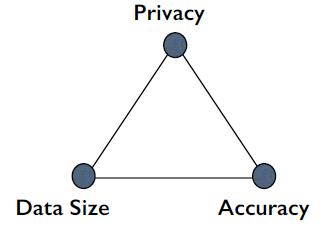
\includegraphics[width=0.3\textwidth]{figures/priacy_data_accuracy.jpg}
    \caption{the relationship of data size, priacy and accuracy}
\end{figure}
\begin{itemize}
    \item \emph{输入扰动 Input perturbation} 输入扰动在获取数据时直接为数据添加上噪声,之后的计算基于添加了噪声的数据。优点:易于实现,可重复使用经过消毒的数据集。\cite{DJW13,KTS17}
    \item \emph{目标扰动 Objective Perturbation} 目标扰动在目标函数中添加一个随机量,以导出最终模型输出的随机性,对目标做随机逼近:随机性取决于J(w)的敏感性属性。 \cite{CMS11,ZZXYW12}
    \item \emph{优化扰动 optimization Perturbation} 优化扰动在执行最小化的过程中,设计满足于差分隐私的优化算法
    \item \emph{输出扰动 Output Perturbation } 输出扰动是最简单直接的Laplace Mechanism思路延续下来的方法,基于输出(模型参数)的敏感度对模型添加噪声,不需要重新设计的基线算法. \cite{CMS11,RBHT12}
\end{itemize}
 
\begin{figure}
    \centering
    \label{fig:estimation_prediction}
    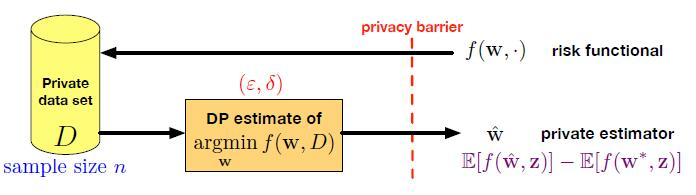
\includegraphics[width=0.7\textwidth]{figures/estimation_prediction.jpg}
    \caption{Statistical estimation}
\end{figure}

统计估计:根据未来数据的良好预期性能,估计一个参数或预测指标。
目标:良好的隐私样本大小权衡
隐私 差分隐私对数据分配没有任何假设:隐私是无条件的。
准确度-准确度度量, 也即“真正的人口分配”:预期的过度统计风险。


$w^* =\min_w \frac{1}{n} \Sigma_{i=1}^n \ell(w,(x_i,y_i)) + \lambda R(w)$
其中  $\lambda R(w)$为抑制过拟合的正则项.


\paragraph{差分隐私优化算法}

\begin{itemize}
\item大数据集是优化的挑战:批(batch)方法不可行
\item使用更多的数据可以帮助我们更好权衡:更好的隐私和准确性
\item在线学习涉及多个版本:可能会有更多的隐私损失
\end{itemize}


目标:使用优化算法保证隐私
机器学习中常见的经验损失最小化方法

$$w^* =\min_w \frac{1}{n} \Sigma_{i=1}^n \ell(w,(x_i,y_i)) + \lambda R(w)$$
中  $\lambda R(w)$为抑制过拟合的正则项.


Non-private SGD 非隐私差分梯度下降

$J(w)=\frac{1}{n} \Sigma_{i=1}^n \ell(w,(x_i,y_i)) + \lambda R(w)$
加噪的隐私随机梯度下降

 


\paragraph{ 实践中遇到的问题}

\begin{itemize}
    \item  Theoretical analysis is for fixed privacy parameters –how should we choose them in practice?
    \item Given a data set, can I tell what the privacy-utilitysample-size tradeoff is?
\item What about more general optimization problems/algorithms?
\item What about scaling (computationally) to large data sets?
\end{itemize}